
\section{概形可视化：幂零元}

\epigraph
  {隐喻的代价，是永远的警惕。}
  {——A.~Rosenbluth 与 N.~Wiener（[Lew, p.~4] 如此归名）}

在 \S3.3 中，我们讨论了如何把\trScheme{}的\trUnderlyingSet{}可视化：在我们先前
关于「传统的点」（即\trClosedPoint）的直观之上添入了\trGenericPoint。其后关于%
\trZariskiTopology{}的讨论与这幅图景吻合得很好。在我们对「\trAffineScheme{}」%
$(\Spec A,\,\OO_{\Spec A})$ 的定义中，还多出了\trNilpotent{}元所携带的一份附加
信息，它们在点的层面上不可见（\S3.2.12），于是现在我们就来弄清如何把它们画出来。
一旦适当的定义就位，我们随即就能把它们粘合起来，画出一般的\trScheme{}的图画。
既然我们是在搭建直观，便不可能做到严格或精确。

作为动机，注意我们有下面这些反转包含关系的双射：
\[
\begin{array}{lcl@{\qquad\qquad}l}
\text{$A$ 的\trMaximalIdeal} & \longleftrightarrow &
  \text{$\Spec A$ 的\trClosedPoint，} &
  \text{（\cref{ex:closed-points-maximal-ideals}）}\\[12pt]
\text{$A$ 的\trPrimeIdeal} & \longleftrightarrow &
  \text{$\Spec A$ 的\trIrreducible{}\trClosedSubset，} &
  \text{（\cref{ex:irreducible-prime-bijection}）}\\[12pt]
\text{$A$ 的\trRadicalIdeal} & \longleftrightarrow &
  \text{$\Spec A$ 的\trClosedSubset。} &
  \text{（\cref{thm:closed-subsets-radical-ideals}）}
\end{array}
\]
若把右边一栏的东西当作「图画」，我们的目标便是弄明白：如何为那些非根的%
\trIdeal{}作画：
\[
\text{$A$ 的\trIdeal} \longleftrightarrow \text{？？？}
\]
（日后我们会以另一种方式把此处严格补全，即引入\emph{\trClosedSubscheme{}}（closed
subscheme）的概念——\trClosedSubset{}的「概形论」版本，见 \S9.1。但我们眼下的
目标只是造出一幅图画。）

作为动机，当我们见到 $\Spec \mathbb{C}[x]/\bigl(x(x-1)(x-2)\bigr)$ 这个表达式时，
会立刻把它解读为 $\mathbb{A}^1_{\mathbb{C}}$ 的一个\trClosedSubset，即
$\{0,\,1,\,2\}$。特别地，映射
$\mathbb{C}[x]\to\mathbb{C}[x]/\bigl(x(x-1)(x-2)\bigr)$ 可以（经中国剩余定理）
解读为：取 $\mathbb{A}^1$ 上的一个函数，并把它限制到三个点 $0$、$1$ 与 $2$ 上。

这将指引我们如何将一个非根\trIdeal{}可视化。最简单的例子是
$\Spec \mathbb{C}[x]/(x^2)$（\cref{ex:small-schemes-dual-numbers}(a)）。作为
$\mathbb{A}^1$ 的子集，它恰是原点 $0=[(x)]$——我们习惯把它想成
$\Spec \mathbb{C}[x]/(x)$（即对应于\trIdeal{} $(x)$，而非 $(x^2)$）。我们想以
某种方式丰富这幅图画。我们应当依据「商记住了哪些信息」来画
$\mathbb{C}[x]/(x^2)$：多项式 $f(x)$ 的\trImage，就是「它在 $0$ 处的值」与「它的导数」
这一信息（参看\cref{ex:derivatives-dual-numbers}）。于是我们把它画成那个点、
再多上一点点——点上的一点无穷小「\trFuzz{}」（fuzz）（见图~\ref{fig:quotients-of-cx}）。
限制序列 $\mathbb{C}[x]\to\mathbb{C}[x]/(x^2)\to\mathbb{C}[x]/(x)$ 应当被解读为
层层嵌套的图画：
\[
\mathbb{C}[x] \twoheadrightarrow \mathbb{C}[x]/(x^2) \twoheadrightarrow \mathbb{C}[x]/(x),
\]
\[
f(x) \longmapsto f(0).
\]
同样，$\mathbb{C}[x]/(x^3)$ 记住的信息还要更多——二阶导数也在其中。于是我们把它
画成带有更多\trFuzz{}的点 $0$。

\begin{figure}[htbp]
\centering
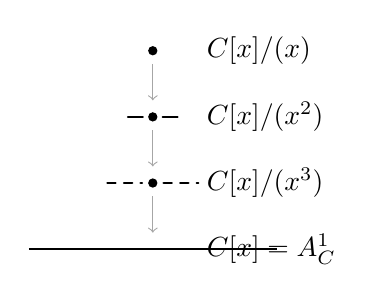
\begin{tikzpicture}[scale=1.05]
  \fill (0,0) circle (1.6pt);
  \node[right=16pt] at (0,0) {$\Spec \mathbb{C}[x]/(x)$};
  \draw[gray!70,->] (0,-0.16) -- (0,-0.60);
  \fill (0,-0.80) circle (1.6pt);
  \draw[thick,line cap=round] (-0.30,-0.80) -- (-0.12,-0.80);
  \draw[thick,line cap=round] (0.12,-0.80) -- (0.30,-0.80);
  \node[right=16pt] at (0,-0.80) {$\Spec \mathbb{C}[x]/(x^2)$};
  \draw[gray!70,->] (0,-0.96) -- (0,-1.40);
  \fill (0,-1.60) circle (1.6pt);
  \draw[thick,dashed,line cap=round] (-0.55,-1.60) -- (-0.13,-1.60);
  \draw[thick,dashed,line cap=round] (0.13,-1.60) -- (0.55,-1.60);
  \node[right=16pt] at (0,-1.60) {$\Spec \mathbb{C}[x]/(x^3)$};
  \draw[gray!70,->] (0,-1.76) -- (0,-2.20);
  \draw[thick] (-1.5,-2.40) -- (1.5,-2.40);
  \node[right=16pt] at (0,-2.40) {$\Spec \mathbb{C}[x]=\mathbb{A}^1_{\mathbb{C}}$};
\end{tikzpicture}
\caption{$\mathbb{C}[x]$ 诸商环的图画。（依原书手绘图重绘。）}%
\label{fig:quotients-of-cx}
\end{figure}

更多的微妙之处出现在二维情形（见图~\ref{fig:quotients-of-cxy}）。考虑
\[
\Spec \mathbb{C}[x,y]/(x,y)^2,
\]
它夹在两个我们十分熟悉的\trRing{}之间：
\[
\mathbb{C}[x,y] \twoheadrightarrow \mathbb{C}[x,y]/(x,y)^2 \twoheadrightarrow \mathbb{C}[x,y]/(x,y),
\]
\[
f(x,y) \longmapsto f(0,0).
\]
同样，对 $(x,y)^2$ 取商记住了「沿一切方向」的一阶导数。我们把它画成围绕该点的%
\trFuzz{}，形状是一个圆（没有任何方向享有特权）。类似地，$(x,y)^3$ 记住了「沿一切
方向」的二阶导数——更大的一圈圆形\trFuzz{}。

\begin{figure}[htbp]
\centering
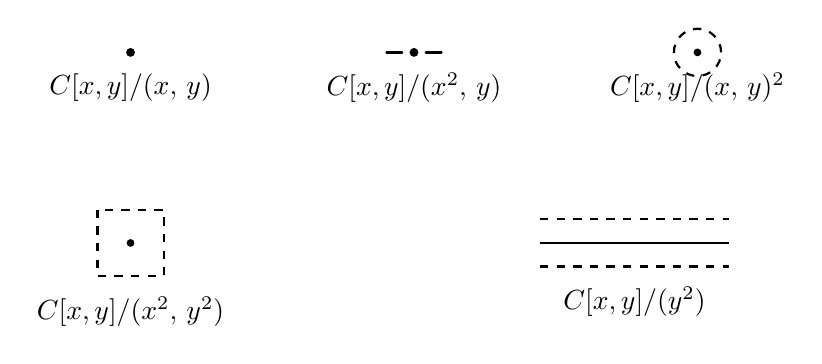
\begin{tikzpicture}[scale=1.0]
  \fill (0,0) circle (1.6pt);
  \node[below=4pt] at (0,0) {$\Spec \mathbb{C}[x,y]/(x,\,y)$};
  \fill (3.6,0) circle (1.6pt);
  \draw[thick,line cap=round] (3.25,0) -- (3.45,0);
  \draw[thick,line cap=round] (3.75,0) -- (3.95,0);
  \node[below=4pt] at (3.6,0) {$\Spec \mathbb{C}[x,y]/(x^2,\,y)$};
  \draw[thick,dashed] (7.2,0) circle (0.30);
  \fill (7.2,0) circle (1.4pt);
  \node[below=4pt] at (7.2,0) {$\Spec \mathbb{C}[x,y]/(x,\,y)^2$};
  \draw[thick,dashed] (-0.42,-2.0) rectangle (0.42,-2.84);
  \fill (0,-2.42) circle (1.4pt);
  \node[below=4pt] at (0,-2.84) {$\Spec \mathbb{C}[x,y]/(x^2,\,y^2)$};
  \draw[thick,dashed] (5.2,-2.12) -- (7.6,-2.12);
  \draw[thick] (5.2,-2.42) -- (7.6,-2.42);
  \draw[thick,dashed] (5.2,-2.72) -- (7.6,-2.72);
  \node[below=4pt] at (6.4,-2.72) {$\Spec \mathbb{C}[x,y]/(y^2)$};
\end{tikzpicture}
\caption{$\mathbb{C}[x,y]$ 诸商环的图画。（依原书手绘图重绘。）}%
\label{fig:quotients-of-cxy}
\end{figure}

换作考虑\trIdeal{} $(x^2,\,y)$。它记住的只是沿 $x$ 方向的导数——给定一个多项式，
我们记住它在 $0$ 处的值，以及 $x$ 的系数。我们画出的\trFuzz{}便只沿 $x$ 方向，以此把
这些信息记住。

至此，我们对给更多这一类东西作画已有了一些抓手，但它如今更像一门艺术，而非一门
科学。比如说，$\Spec \mathbb{C}[x,y]/(x^2,\,y^2)$ 或许可以画成原点四周一块
毛茸茸的正方形。（你能相信这个正方形既内接于圆形\trFuzz{}
$\Spec \mathbb{C}[x,y]/(x,y)^3$、又外接于圆形\trFuzz{}
$\Spec \mathbb{C}[x,y]/(x,y)^2$ 吗？）这个例子的一个特征是：给定一个\trRing{} $A$
（比如 $\mathbb{C}[x,y]$）的两个\trIdeal{} $I$ 与 $J$，你对 $\Spec A/(I,\,J)$
的毛茸茸图画，应当是你关于 $\Spec A/I$ 与 $\Spec A/J$ 在 $\Spec A$ 中的图画
二者的「相交」。（你将在练习~9.1.I(a) 中把这一点弄精确。）比如说，
$\Spec \mathbb{C}[x,y]/(x^2,\,y^2)$ 应当是两条加厚直线之交。（你会如何画
$\Spec \mathbb{C}[x,y]/(x^5,\,y^3)$？$\Spec \mathbb{C}[x,y,z]/(x^3,\,y^4,\,z^5,\,(x+y+z)^2)$？
$\Spec \mathbb{C}[x,y]/\bigl((x,y)^5,\,y^3\bigr)$？）

最后一个例子将在 \S6.6 中激励我们：$\Spec \mathbb{C}[x,y]/(y^2,\,xy)$。知道
$\mathbb{C}[x,y]$ 中的多项式模 $(y^2,\,xy)$ 后是什么，就等价于既知道它在
$x$-轴上的取值，又知道原点附近的一阶微分信息。这值得仔细想透：你能在
图~\ref{fig:nonreduced-y2xy} 中（纵使并不完美地）看出这些信息是如何被捕捉的吗？

\begin{figure}[htbp]
\centering
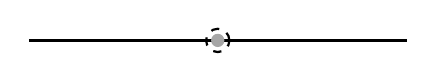
\begin{tikzpicture}[scale=1.0]
  \draw[thick] (-2.4,0) -- (2.4,0);
  \fill[gray!70] (0,0) circle (2.4pt);
  \draw[thick,dashed] (0,0) circle (4.2pt);
\end{tikzpicture}
\caption{$\Spec k[x,y]/(y^2,\,xy)$ 这个\trScheme{}的一幅图。原点处的\trFuzz{}标示出
「非\trReduced{}性」位于何处。（依原书手绘图重绘。）}%
\label{fig:nonreduced-y2xy}
\end{figure}

我们的图画捕捉到了一些你已经对其抱有直观的有用信息。比如说，考虑抛物线
$y=x^2$ 与 $x$-轴（在 $xy$ 平面中）的相交；见图~\ref{fig:scheme-theoretic-intersection}。
你已经有这样的感觉：这个相交的\trMultiplicity{}是 $2$。用这种可视化语言来说，我们把这个交
解读为（在 $\Spec \mathbb{C}[x,y]$ 中的）一次相交：
\begin{align*}
\Spec \mathbb{C}[x,y]/(y-x^2) \cap \Spec \mathbb{C}[x,y]/(y)
  &= \Spec \mathbb{C}[x,y]/(y-x^2,\,y)\\
  &= \Spec \mathbb{C}[x,y]/(y,\,x^2),
\end{align*}
我们把这解读为如下事实：抛物线与这条直线不只是以\trMultiplicity{} $2$ 相遇，而且「\trMultiplicity{} $2$」
这一部分是沿 $x$-轴方向的。你将在练习~9.1.I(b) 中把这个例子弄精确。

\begin{figure}[htbp]
\centering
\begin{tikzpicture}[scale=1.0]
  \draw[thick] plot[domain=-0.75:0.75] (\x,{1.9*\x*\x});
  \node at (2.1,0.55) {相交};
  \draw[thick] (3.2,0.55) -- (4.6,0.55);
  \node at (5.15,0.55) {$=$};
  \draw[line width=2.2pt] (5.9,0.55) -- (6.3,0.55);
\end{tikzpicture}
\caption{抛物线 $y=x^2$ 与 $x$-轴的「概形论」相交是一个非\trReduced{}\trScheme%
（\trFuzz{}沿 $x$ 方向）。（依原书手绘图重绘。）}%
\label{fig:scheme-theoretic-intersection}
\end{figure}

\textbf{4.2.1.}\quad 日后在讨论\trAssociatedPoint{}（associated points）时，我们会把\trFuzz{}的
位置说得更加精确。届时将看到：在合理的情形下，\trFuzz{}集中在\trClosedSubset{}上
（练习~6.6.N）。

\epigraph
  {人们一再地说，几何是在画得糟糕的图形上作良好推理的艺术；然而这些图形若要不
   欺骗我们，就必须满足一定的条件：各部分之间的比例可以被大幅度地改动，但各个
   部分的相对位置却不容搅乱。}
  {——\trn{H.~Poincar\'e}{\trPoincare{}}，[Po1, p.~2]（参看 J.~Stillwell 的英译
   [Po2, p.~ix]）}
